\chapter{辅助图表}

\section{有关中微子源的显著性分析的其他图表}
\label{appendix:sensitivity_plots}

\begin{figure}[!htb]%
    \centering
    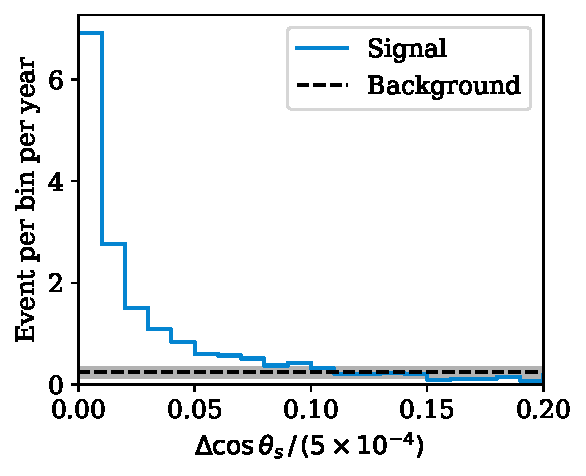
\includegraphics[width=0.55\textwidth]{img/event_rate_around_source_3.2TeV.pdf}
    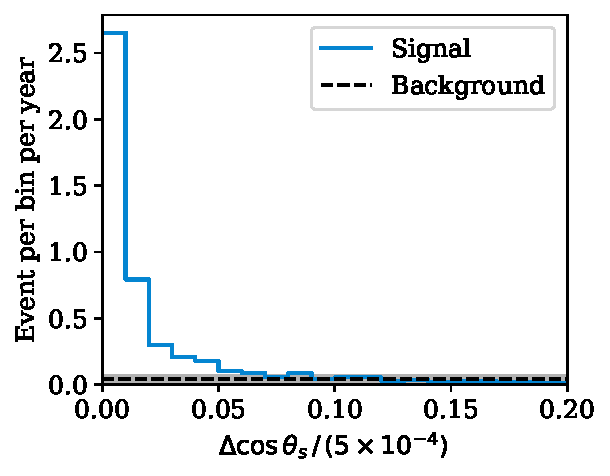
\includegraphics[width=0.55\textwidth]{img/event_rate_around_source_10TeV.pdf}
    \caption{
    不同的中微子能量阈值下,重建得到的信号和背景事件在源附近的立体角空间上的事例率分布图。
    上图的阈值为$3.2\,\mathrm{TeV}$,下图为$10\,\mathrm{TeV}$。
    }
    \label{fig:event_rate_around_source_energy_threshold}
\end{figure}

\section{有关阵列的几何构型的其他图表}
\label{appendix:geometry_plot}

\begin{figure}[!htb]%
    \centering
    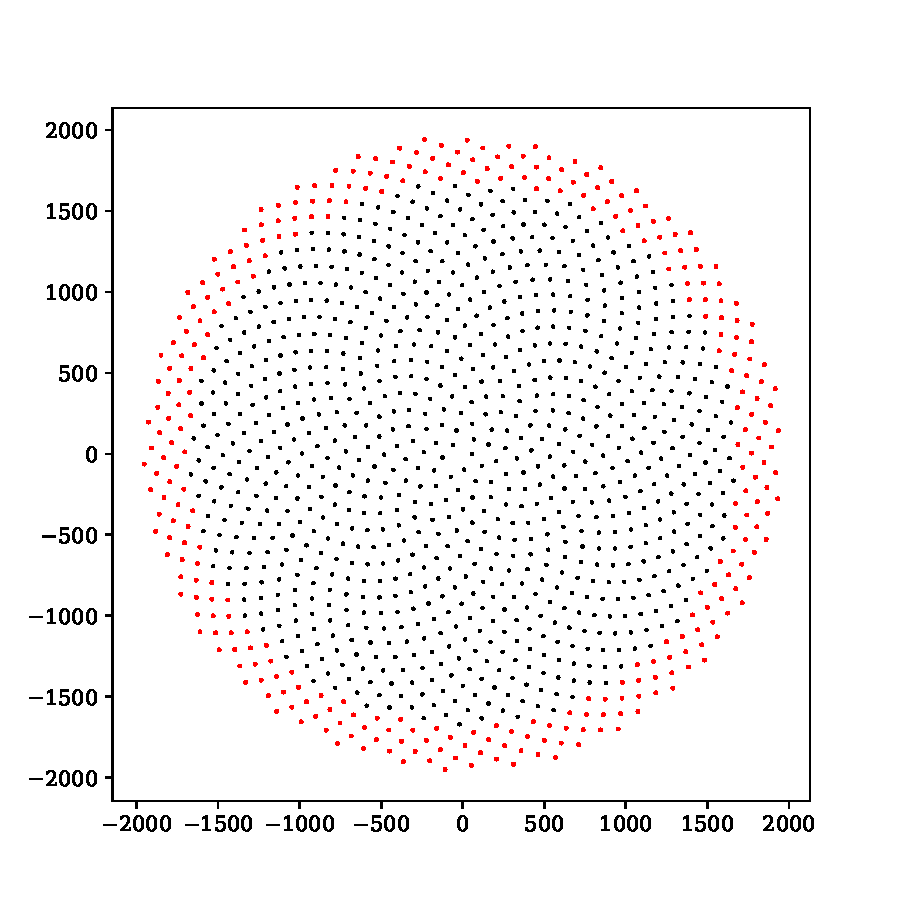
\includegraphics[width=0.80\textwidth]{img/geo_layout_sunflower.pdf}
    \caption{向日葵构型下,串列单元在水平方向上的排布。每一个点表示一根串列单元,其中红色加粗的点表示在外围用于屏蔽的串列单元。}
    \label{fig:geo_layout_sunflower}
\end{figure}

\begin{figure}[!htb]%
    \centering
    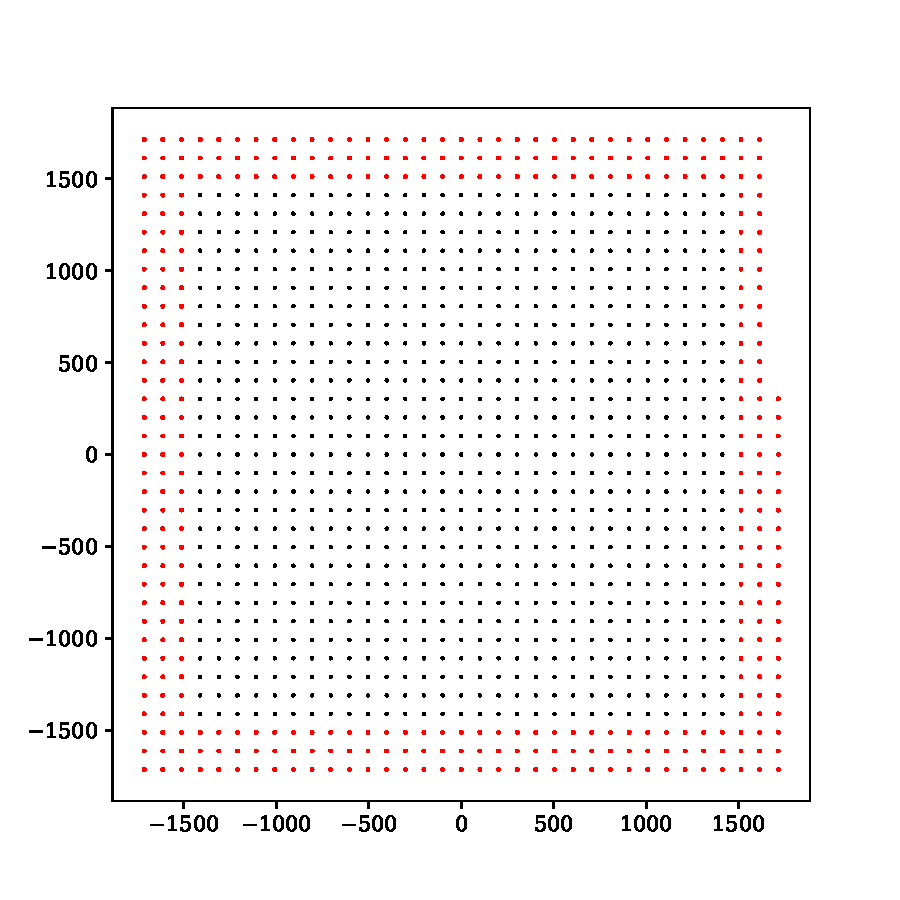
\includegraphics[width=0.80\textwidth]{img/geo_layout_cube.pdf}
    \caption{正方形构型下,串列单元在水平方向上的排布。每一个点表示一根串列单元,其中红色加粗的点表示在外围用于屏蔽的串列单元。}
    \label{fig:geo_layout_cube}
\end{figure}

\begin{figure}[!htb]%
    \centering
    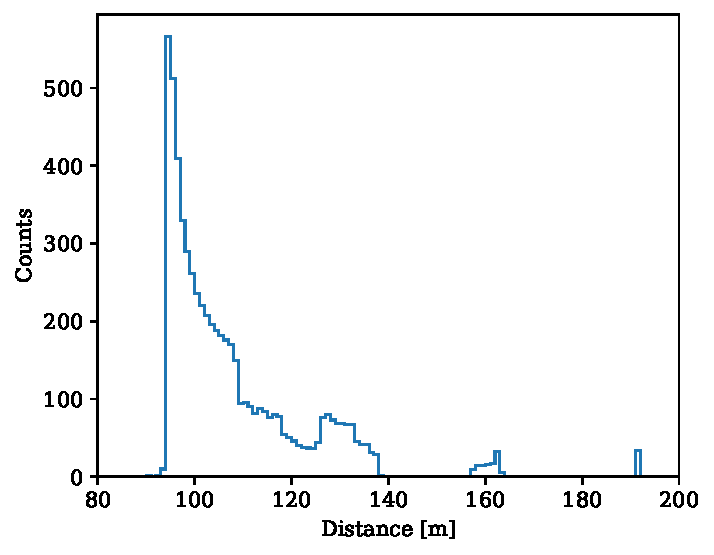
\includegraphics[width=0.65\textwidth]{img/distance_spectrum_sunflower.pdf}
    \caption{向日葵构型中串列单元之间的水平间距分布图。}
    \label{fig:distance_spectrum_sunflower}
\end{figure}

\begin{figure}[!htb]%
    \centering
    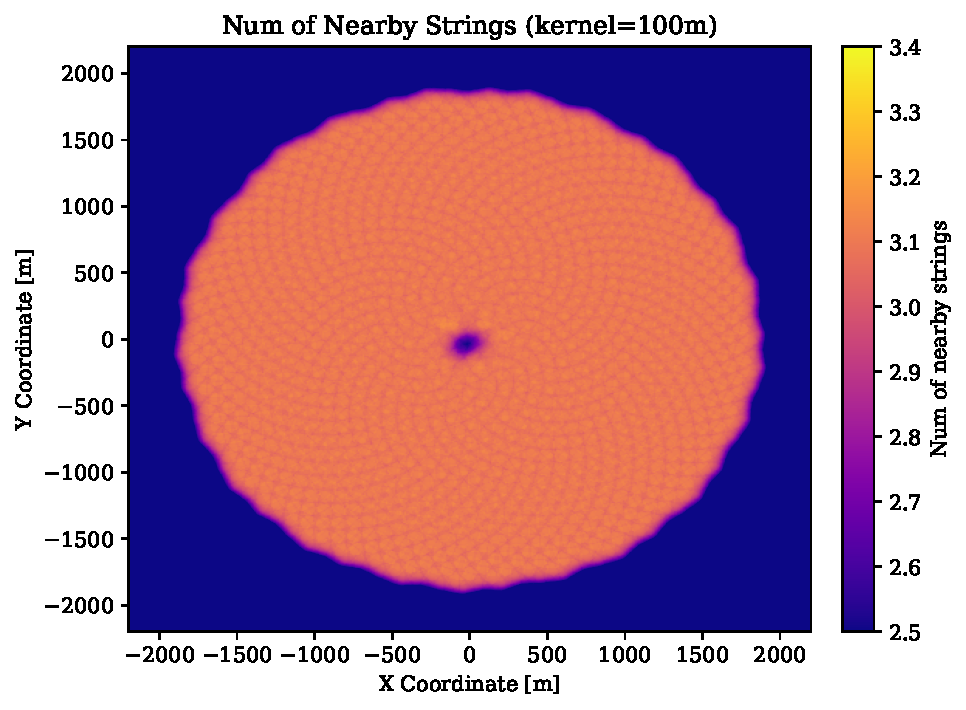
\includegraphics[width=0.85\textwidth]{img/string_density_sunflower.pdf}
    \caption{在观测的分辨率为一个$sigma = 100\,\mathrm{m}$的二维高斯函数的情况下,观测到向日葵构型的串列单元的密度分布。}
    \label{fig:string_density_sunflower}
\end{figure}

\begin{figure}[!htb]%
    \centering
    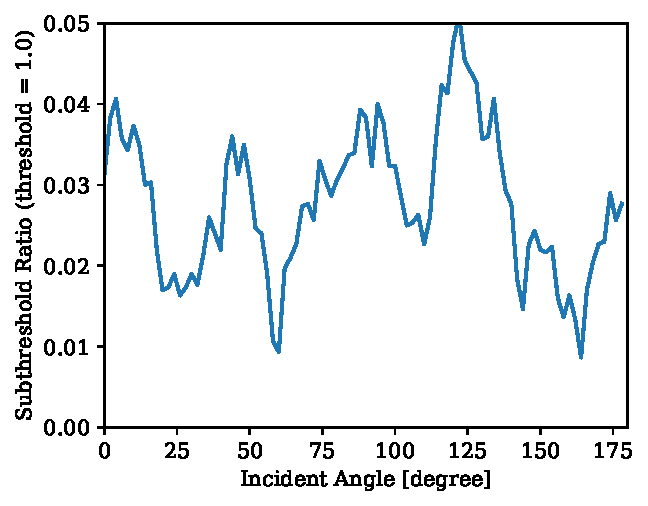
\includegraphics[width=0.60\textwidth]{img/corridor_angle_sunflower.pdf}
    \caption{向日葵构型下,缪子事件对屏蔽层的逃逸率与缪子入射角度的关系图。}
    \label{fig:corridor_angle_sunflower}
\end{figure}

\begin{figure}[!htb]%
    \centering
    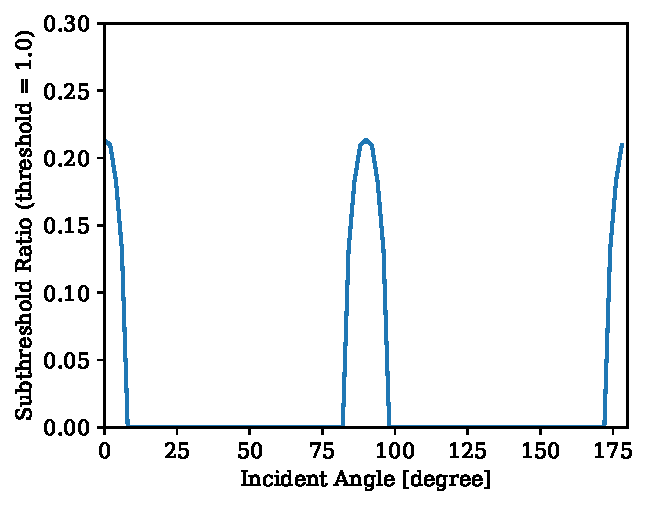
\includegraphics[width=0.60\textwidth]{img/corridor_angle_cube.pdf}
    \caption{正方形构型下,缪子事件对屏蔽层的逃逸率与缪子入射角度的关系图。}
    \label{fig:corridor_angle_cube}
\end{figure}

\section{有关阵列间距的其他图表}

\begin{figure}[!htb]%
    \centering
    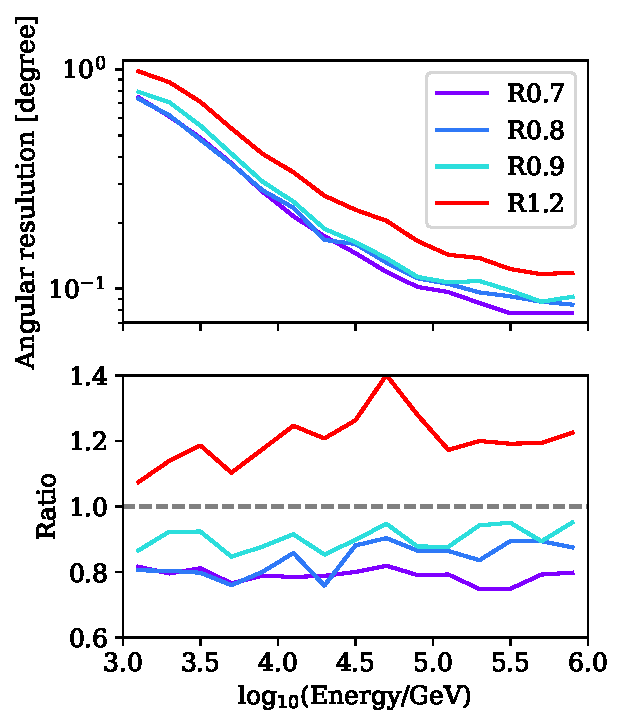
\includegraphics[width=0.45\textwidth]{img/spacing/angular_resuolution_hori.pdf}
    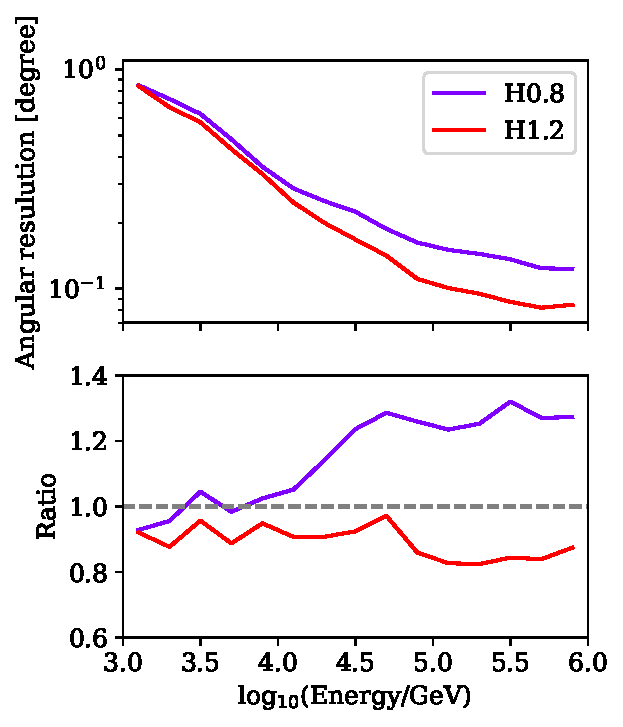
\includegraphics[width=0.45\textwidth]{img/spacing/angular_resuolution_vert.pdf}
    \caption{不同的阵列几何间距下,海铃对缪子径迹型事件的角分辨的变化。左图表示对水平缩放因子的分析,而右图表示对垂直缩放因子的分析;上图表示绝对角分辨率,而下图表示相对于标准整列配置的角分辨变化。其中红色线表示放大阵列的水平或者垂直间距,而蓝紫色线表示缩小阵列的间距,具体的放大因子参见图注。}
    \label{fig:spacing_angular_resuolution}
\end{figure}

\begin{figure}[!htb]%
    \centering
    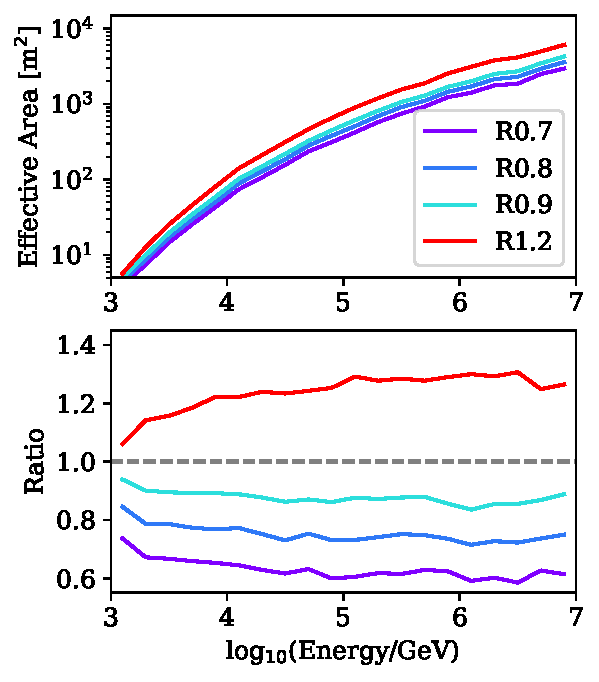
\includegraphics[width=0.45\textwidth]{img/spacing/effective_area_horizontal_hori.pdf}
    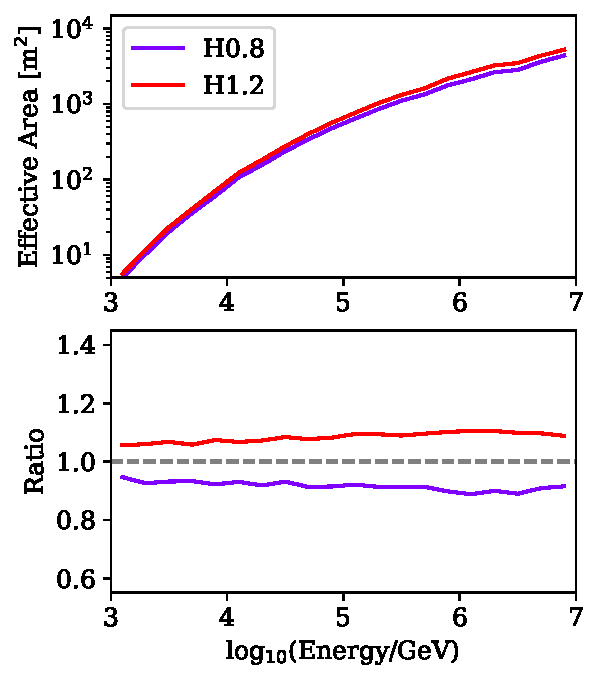
\includegraphics[width=0.45\textwidth]{img/spacing/effective_area_horizontal_vert.pdf}
    \caption{与图\ref{fig:spacing_angular_resuolution}类似,但是表示海铃对来自水平方向的缪子径迹型事件的有效面积。}
    \label{fig:spacing_effective_area_horizontal}
\end{figure}

\begin{figure}[!htb]%
    \centering
    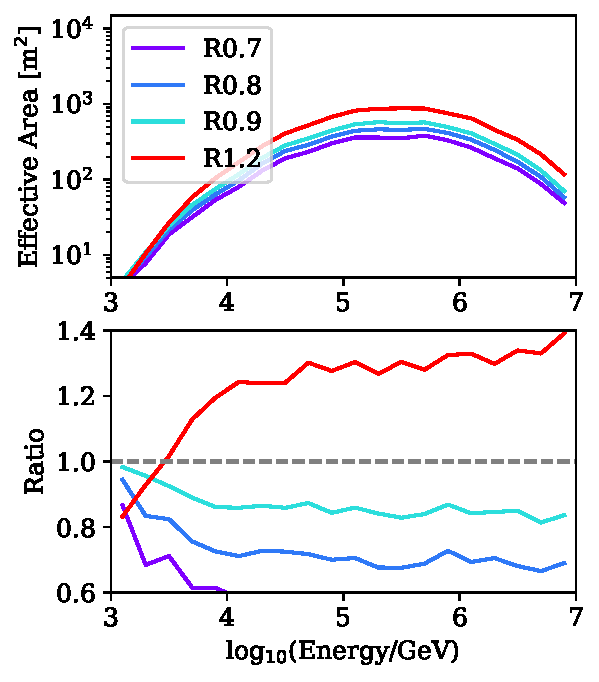
\includegraphics[width=0.45\textwidth]{img/spacing/effective_area_up-going_hori.pdf}
    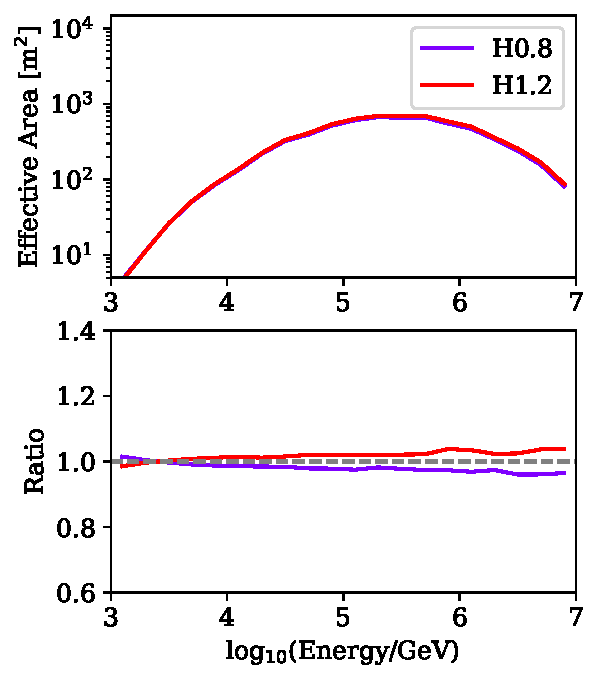
\includegraphics[width=0.45\textwidth]{img/spacing/effective_area_up-going_vert.pdf}
    \caption{与图\ref{fig:spacing_angular_resuolution}类似,但是表示海铃对向上穿行的缪子径迹型事件的有效面积。}
    \label{fig:spacing_effective_area_up-going}
\end{figure}
